\textbf{Ejercicio 28.} Calcular el volumen de la región limitada por
\[
x^2 + y^2 = 4x, \quad z = x, \quad z = 3x.
\]

Comenzamos reescribiendo la ecuación
\[
x^2 + y^2 = 4x \;\;\Longleftrightarrow\;\; x^2 - 4x + y^2 = 0
\]
\[
(x - 2)^2 + y^2 = 4.
\]


La región queda entonces descripta como un cilindro de radio \(2\) centrado en \((2,0)\), intersectado por los planos
\[
z = x \quad \text{y} \quad z = 3x.
\]

\bigskip

\begin{figure}[h]
\centering
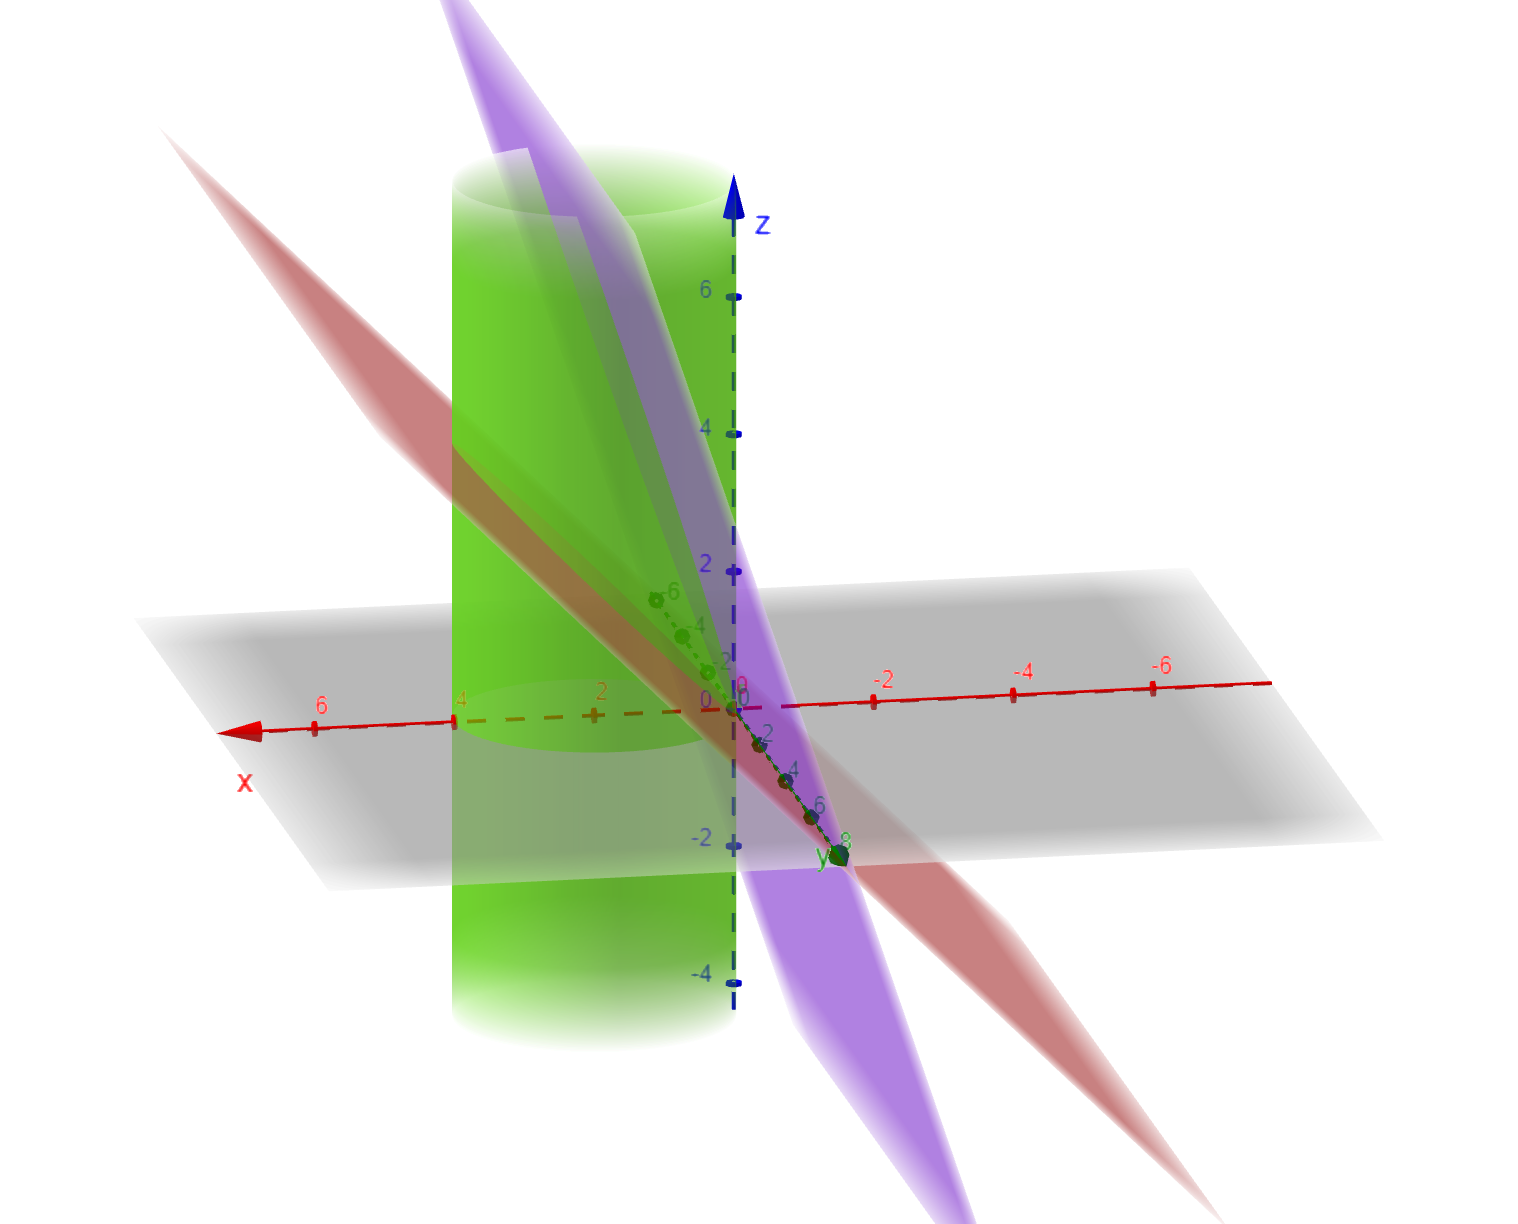
\includegraphics[width=0.6\textwidth]{ejercicios/ejercicio28.png}
\caption{Representación de la región pedida.  \href{https://www.geogebra.org/m/uhgycge3}{Ver en GeoGebra}}
\centering
\end{figure}

Para describir la región, utilizamos coordenadas cilíndricas trasladadas:
\[
x = 2 + r\cos\theta, \quad y = r\sin\theta,
\]
con
\[
0 \leq r \leq 2, \qquad 0 \leq \theta \leq 2\pi.
\]

En estas coordenadas, las cotas para \(z\) resultan:
\[
z = 2 + r\cos\theta, \qquad z = 3(2 + r\cos\theta),
\]
es decir,
\[
2 + r\cos\theta \leq z \leq 6 + 3r\cos\theta.
\]

El jacobiano del cambio de variables es
\[
dV = r \, dz \, dr \, d\theta.
\]

Luego, el volumen se expresa como
\[
V = \int_0^{2\pi} \int_0^2 \int_{2 + r\cos\theta}^{6 + 3r\cos\theta} r \, dz \, dr \, d\theta.
\]


\[
V = \int_0^{2\pi} \int_0^2 r \big(4 + 2r\cos\theta\big) \, dr \, d\theta,
\]
\[
V = \int_0^{2\pi} \int_0^2 \big(4r + 2r^2\cos\theta\big) \, dr \, d\theta.
\]

\[
V = \int_0^{2\pi} \left(8 + \frac{16}{3}\cos\theta\right) d\theta.
\]

Finalmente,
\[
\boxed{V = 16\pi}
\]
